% -*- mode: fundamental -*-

% ****************************************************************

\chapter{Overview of the RISC-V ISA}

\markboth{Ch \arabic{chapter}: RISC-V ISA Overview (DRAFT)}{\copyrightnotice}


\setcounter{page}{1}
% \renewcommand{\thepage}{\arabic{page}}
\renewcommand{\thepage}{\arabic{chapter}-\arabic{page}}

\label{ch_ISA}

% ****************************************************************

\section{What is an ISA?}

\index{RISC-V!ISA!Instruction Set Architecture}

The acronym ``ISA'' stands for ``Instruction Set Architecture''.
Figure~\ref{Fig_What_is_an_ISA} illustrates the role of an ISA as an
intermediary between hardware (CPU implementations) and software
(which runs on the CPU hardware).
\begin{figure}[htbp]
  \centerline{\includegraphics[width=6in,angle=0]{Figures/Fig_What_is_an_ISA}}
  \caption{\label{Fig_What_is_an_ISA} What is an ISA?}
\end{figure}

An ISA, \emph{per se}, is neither software nor hardware.  It is merely
a \emph{specification}, a document defining three things:

\begin{itemize}

  \index{RISC-V!ISA!Architectural State}
  \index{RISC-V!ISA!Program Counter, PC}
  \index{RISC-V!ISA!PC, Program Counter}
  \index{RISC-V!ISA!Register File}

  \item \emph{Architectural State}: the registers visible to the
        instructions, such as the program counter (PC) and a register
        file containing, say, 32 registers named x0 through x31.

        Typically (nowadays), the architectural state includes a
        \emph{byte-addressed} memory (a memory where an \emph{address}
        identifies a single byte, and where individual bytes may be
        read and written.

  \index{RISC-V!ISA!Instruction Set}
  \index{RISC-V!ISA!Instruction Set encoding in bits}
  \index{RISC-V!ISA!Assembly Language}

  \item An \emph{Instruction Set}: a collection of instructions.  For
        each instruction, the ISA specifies how it is encoded in bits.
        The ISA may also specify a way of writing an instruction in
        symbolic text, which we call Assembly Language.  Instructions
        are typically grouped in classes, such as Immediate,
        LOAD/STORE, Arithmetic and Logic, Conditional Branches, Jumps,
        System Instructions, and so on.

  \index{RISC-V!ISA!Instruction semantics}

  \item \emph{Semantics}: a description, for each instruction about
        \emph{how} it executes---what architectural state it observes,
        and what architectural state it updates, and how.  For
        example, a Conditional Branch instruction typically observes
        two registers in the register file, compares them, and updates
        the PC depending on the comparison result.

        The overal semantics of a program being executed is just a
        sequential composition of individual instruction semantics.

\end{itemize}

\index{RISC-V!ISA!Formal Specification in Sail}
\index{RISC-V!ISA!Sail Formal Specification language}

The full ISA may be described in ordinary text prose and diagrams, or
in a semi-formal or formal language.  For example, the RISC-V ISA is
described both in text prose and diagrams, and in the formal language
``Sail''.

\index{RISC-V!Micro-architecture}
\index{RISC-V!Micro-architecture!Superscalar}
\index{RISC-V!Micro-architecture!Out-of-order}
\index{RISC-V!Micro-architecture!Pipelining}
\index{RISC-V!Micro-architecture!Speculation}
\index{RISC-V!Micro-architecture!Multi-threaded}
\index{RISC-V!Micro-architecture!Multi-core}

Beneath the ISA level are actual \emph{implementations} of the ISA.
These range from software simulators of the ISA to silicon
implementations.  Silicon implementations typically vary widely in
their \emph{micro-architecture} features, such as pipelining, in-order
or out-of-order, speculation, superscalarity, multi-threading,
multi-core.  The choice of micro-architecture is typically based on a
particular target market, trading-off cost, performance (speed),
energy consumption, capabilities (embedded software to full server OS
with network and storage stacks), silicon technology (FPGA {\vs} ASIC,
ASICs with various silicon feature sizes and techniques), and so on.
Variations in micro-architectures provide product differentiation.

\index{RISC-V!Machine code}

Each implementation runs (interprets) machine code, {\ie} an encoding
of instructions in memory.  The machine codes are typically produced
by compilers, which are themselves machine code programs that
transform source codes into machine codes.  Some machine codes are
themselves software interpreters for so-called interpreted languages
such as Python, Javascript, Java, Scheme, Lisp, and so on.

A crucially important point is that \emph{all the implementations of
an ISA should respect the semantics of the ISA as specified in the ISA
definition}.  They can (and do) play all kinds of micro-architectural
tricks under the covers, but the result of executing any program
should be explainable purely based on the ISA specification.

\index{RISC-V!ISA!Enables software portability}
\index{RISC-V!ISA!Contract between software and hardware implementations}

Thus, and ISA is a \emph{contract} or \emph{API} between software and
hardware implementations.  People writing software, people writing
compilers for software, people writing interpreters for interpreted
languages, {\etc} need only to understand and refer to the ISA
specification to do their job.  They do not need to know about the
specific hardware implementation on which it will eventually run.
This enables \emph{software portability}, {\ie} a machine code program
for an ISA should be able to run, without change, on \emph{any}
implementation of the ISA, including future next-generation
laptops/servers for the ISA.

% ----------------
\vspace{2ex}

NOTE:
\fbox{\small
\begin{minipage}{5in}

In the rarer cases where the ``bleeding edge'' of software performance
really matters, human coders and compilers may produce different
machine codes for specific implementations of the same ISA, in order
to exploit particular quirks of each implementation's
micro-architecture such as branch-prediction or register-hazard
penalties.

\end{minipage}}

\vspace{2ex}
% ----------------

Examples of ISAs include:

\begin{tightlist}

  \item \emph{RISC-V}: Open ISA (not proprietary).  Silicon
        implementations from various vendors, worldwide.

  \item \emph{x86}: Proprietary.  Silicon Implementations from Intel
        and AMD, primarily, with names like Xeon, Core i9, 13th
        Generation Core, Alder Lake, Raptor Lake, and so on.

  \item \emph{ARMv8}, \emph{ARMv9}: Proprietary.  Implementations from
        ARM licensees like Apple, Samsung, Broadcom and others.

  \item \emph{Power}: Proprietary. Implementations from IBM and other
        licensees.

  \item \emph{Sparc}: Proprietary. Implementations originally from Sun
        Microsystems, nowadays from Oracle, and also from licensees
        such as Fujitsu.

  \item \emph{MIPS}: Proprietary. Implementations from MIPS and other
        licensees.

  \item Other famous, but now defunct ISAs: \emph{Alpha} (from Digital
        Equipment Corp./Compaq/HP), \emph{Itanium} (from Intel, HP),
        \emph{68000} and \emph{88000} (from Motorola), ...

\end{tightlist}

% ****************************************************************

\section{Why choose RISC-V?}

In the list of ISAs above, except for RISC-V, all the other ISAs are
\emph{proprietary}, {\ie}, in order to produce and sell a silicon
implementation it is necessary to obtain a license (permission) from
the company that ``owns'' the ISA.  These licenses can be very
expensive, in the thousands of dollars or more.

The RISC-V ISA is owned by RISC-V International (``RVI''), a
non-profit corporation based in Switzerland (\url{https://riscv.org}).
The ISA is ``open'' in that no prior permission or license from RVI is
needed in order to produce and sell implementations of the ISA.  If a
\emph{commercial} product is claimed publicly to implement the RISC-V
ISA, the vendor needs to get official certification from RVI that it
indeed does so (it must pass a battery of certification tests), but
this is a one-time certification, quite different from a production
license.  Non-commercial products (from universities, research labs,
hobbyists, {\etc}) do not need any such certification.

Separate from these commercial concerns, there are also concerns about
quality of an ISA and the richness of the ecosystem supporting an ISA.
The RISC-V ISA is attractive on these dimensions as well.

The RISC-V ISA was originally designed at University of California,
Berkeley, by a team of researchers who have half a century of deep
knowledge and experience on ISAs, computer architectures, computer
systems, and ecosystem software (the Sparc ISA also came out of
Berkeley in the 1980s).  As such, the RISC-V ISA can be seen as a new,
clean-slate design that incorporates all the lessons learned from all
previous ISAs dating all the way back to the 1950s.

An ISA is useless without a strong \emph{ecosystem} supporting the
ISA.  This includes artefacts such as compilers, programming language
implementqtions, debuggers, test and verification infrastructure,
embedded operating systems, real-time operating systems, workstation
and server-class operating systems, boot loaders, device drivers, and
so on.  It also includes services, such as tutorials, books, courses,
and training materials (this book can be seen as a contribution).  The
RISC-V ecosystem is already quite rich, and it grows daily precisely
because of the open nature of the ISA, enabling thousands of
contributors worldwide to participate in the effort.

The openness of the RISC-V ISA also enables entrepreneurs and
researchers to attempt \emph{innovations} in micro-architecture and
design and production techniques, something which is not practically
feasible with a proprietary ISA.

There is also a security dimension to RISC-V's attractiveness.  When a
customer buys a silicon implementation of an ISA, they have to trust
that neither the vendor nor the supply chain inserted any secret
``back-doors'' by which others can monitor what the processor is doing
or, worse, disable it or program it remotely.  The RISC-V ISA being
open, it is more possible for a customer to develop their own trusted
supply chains for silicon implementations.

Silicon implementations of RISC-V are already availble from dozens of
vendors located in several countries worldwide.  These supply chains
are only likely to grow more diverse.  Many production-ready,
competitive RISC-V designs are available in free and open-source form.

% ****************************************************************

\section{Overview of the RISC-V ISA}

RISC-V: RV32 and RV64

RISC-V ISA Modularity: Base + Options

RISC-V ISA Spec Documents .. Sail formal spec

% ================================================================

\subsection{Unprivileged ISA RV32I}

Instruction encodings

Immediate values

RV32I forty instructions overview

How to read the ISA spec: examples LUI, AUIPC, Conditional Branch,
LOAD/STORE, Register-Register Arithmetic and Logic, Register-Immediate
Arithmetic and Logic, Unconditional Jump.

% ================================================================

\subsection{What about illegal instructions?}

ECALL and EBREAK

% ================================================================

\subsection{Assembly Language and Calling Conventions}

% ================================================================

\subsection{Standard Unprivileged ISA Extensions}

M, A, FD, C

% ================================================================

\subsection{RV64I differences from RV32I}

% ================================================================

\subsection{Brief description of privileged ISA}

MSTATUS, MTVEC, MEPC, MTVAL, MCAUSE, ...

% ****************************************************************

\section{Resources}

This chapter contains only generic RISC-V information, not specific to
this book.  This chapter can be safely skipped by those already
familiar with these generic topics, or who choose to learn it
elsewhere:

\begin{itemize}

\item RISC-V ISA specification documents.
      Please see Appendix \ref{apx_resources_ISA_specs} for links.

\item RISC-V Assembly Language manuals
      Please see Appendix \ref{apx_resources_asm_manuals} for links.

\item RISC-V Gnu Tools and related documentation.
      Please see Appendix \ref{apx_resources_gnu_tools} for links.

\item RISC-V textbooks.
      Please see Appendix \ref{apx_resources_RISCV_textbooks} for links.

\end{itemize}

% ****************************************************************
